\chapter{Metodoloxía}
\label{chap:metodoloxia}

O proxecto desenvolveuse mediante un enfoque \textbf{incremental e iterativo}, empregando un taboleiro \textbf{Kanban} para organizar as tarefas e realizar o seu seguimento. Esta forma de traballo permitiu avanzar por etapas, comprobar os resultados de cada unha e adaptar o desenvolvemento ás necesidades que foron aparecendo.

Optouse por un fluxo continuo de traballo, no que as tarefas se priorizaron segundo a súa importancia para o funcionamento principal do sistema, as dependencias existentes, a dificultade e a incerteza técnica e a proximidade dos fitos establecidos.

\section{Enfoque incremental e iterativo}

O desenvolvemento incremental consiste en construír o sistema mediante etapas sucesivas que amplían progresivamente as súas capacidades. Cada incremento parte dos resultados obtidos nos anteriores e incorpora novas funcionalidades ou melloras.

O carácter iterativo permite revisar e modificar solucións xa desenvolvidas cando aparecen novos datos ou necesidades. Isto foi especialmente importante neste proxecto, xa que a estrutura das follas de tratamento, os resultados das técnicas de extracción e os requisitos da aplicación móbil fóronse coñecendo con maior precisión durante o desenvolvemento.

En lugar de desenvolver a aplicación completa desde o principio, o traballo dividiuse en varios pasos. Primeiro estudouse se era posible extraer os datos automaticamente dos documentos, despois desenvolveuse unha API capaz de procesar as follas de tratamento e, finalmente, creouse a aplicación móbil que consume esa API e permite utilizar os resultados.

Esta forma de traballo evitou desenvolver a aplicación móbil arredor dunha tecnoloxía de extracción que podía non ofrecer resultados suficientemente fiables. Ademais, permitiu comprobar o funcionamento de cada compoñente antes de realizar a integración completa do sistema.

Os incrementos concretos nos que se dividiu o desenvolvemento e o seu seguimento temporal descríbense no capítulo (\ref{chap:planificacion}).

\section{Aplicación de Kanban}

Kanban é un método de xestión visual que permite representar as tarefas do proxecto segundo o seu estado. Cada tarefa móvese entre distintas columnas a medida que avanza o seu desenvolvemento, o que facilita coñecer o traballo pendente, identificar as actividades que se están realizando e comprobar as que xa foron completadas.  Para aplicar Kanban no proxecto empregouse un taboleiro de GitHub Projects con catro estados:
\begin{itemize}
    \item \textbf{Para máis adiante:} ideas, melloras ou tarefas que se consideraban útiles, pero que non formaban parte do traballo inmediato.
    \item \textbf{Por facer:} tarefas xa definidas, revisadas e priorizadas que estaban preparadas para comezar.
    \item \textbf{En curso:} tarefas nas que se estaba traballando ou que permanecían pendentes dalgunha comprobación.
    \item \textbf{Feito:} tarefas completadas e comprobadas.
\end{itemize}

Na Figura~\ref{fig:taboleiro-kanban} móstrase o estado do taboleiro
Kanban nun momento do desenvolvemento, coas tarefas
distribuídas segundo o seu estado.

O movemento das tarefas entre as columnas non se realizaba automaticamente. As tarefas situadas en \textit{Para máis adiante} revisábanse periodicamente e trasladábanse a \textit{Por facer} cando pasaban a formar parte dos obxectivos próximos do proxecto. Nese momento comprobábase tamén que estivesen suficientemente definidas e que a prioridade asignada seguise sendo adecuada.

Para iniciar unha nova tarefa seleccionábase unha das actividades da columna \textit{Por facer}, atendendo en primeiro lugar á prioridade que tiña asignada. Cando varias tarefas compartían o mesmo nivel, tíñanse en conta as dependencias con outras actividades, a incerteza técnica e a existencia de posibles bloqueos. Antes de movela a \textit{En curso}, comprobábase tamén que non se superase o límite de traballo establecido.

Unha vez iniciado o traballo, a tarefa permanecía na columna \textit{En curso} durante a súa realización e comprobación. Se para completala era necesario realizar modificacións adicionais, probas ou integracións con outros compoñentes, continuaba nesta columna ata que se resolvesen.

Unha tarefa só se trasladaba a \textit{Feito} despois de cumprir os criterios de aceptación, realizar as comprobacións necesarias e integrar o resultado no proxecto. Deste xeito, a existencia dunha implementación parcial non era suficiente para considerar unha tarefa rematada.

O movemento seguido polas tarefas entre as distintas columnas represéntase na Figura~\ref{fig:diagrama-kanban}.
\FloatBarrier

 \begin{figure}
     \centering
     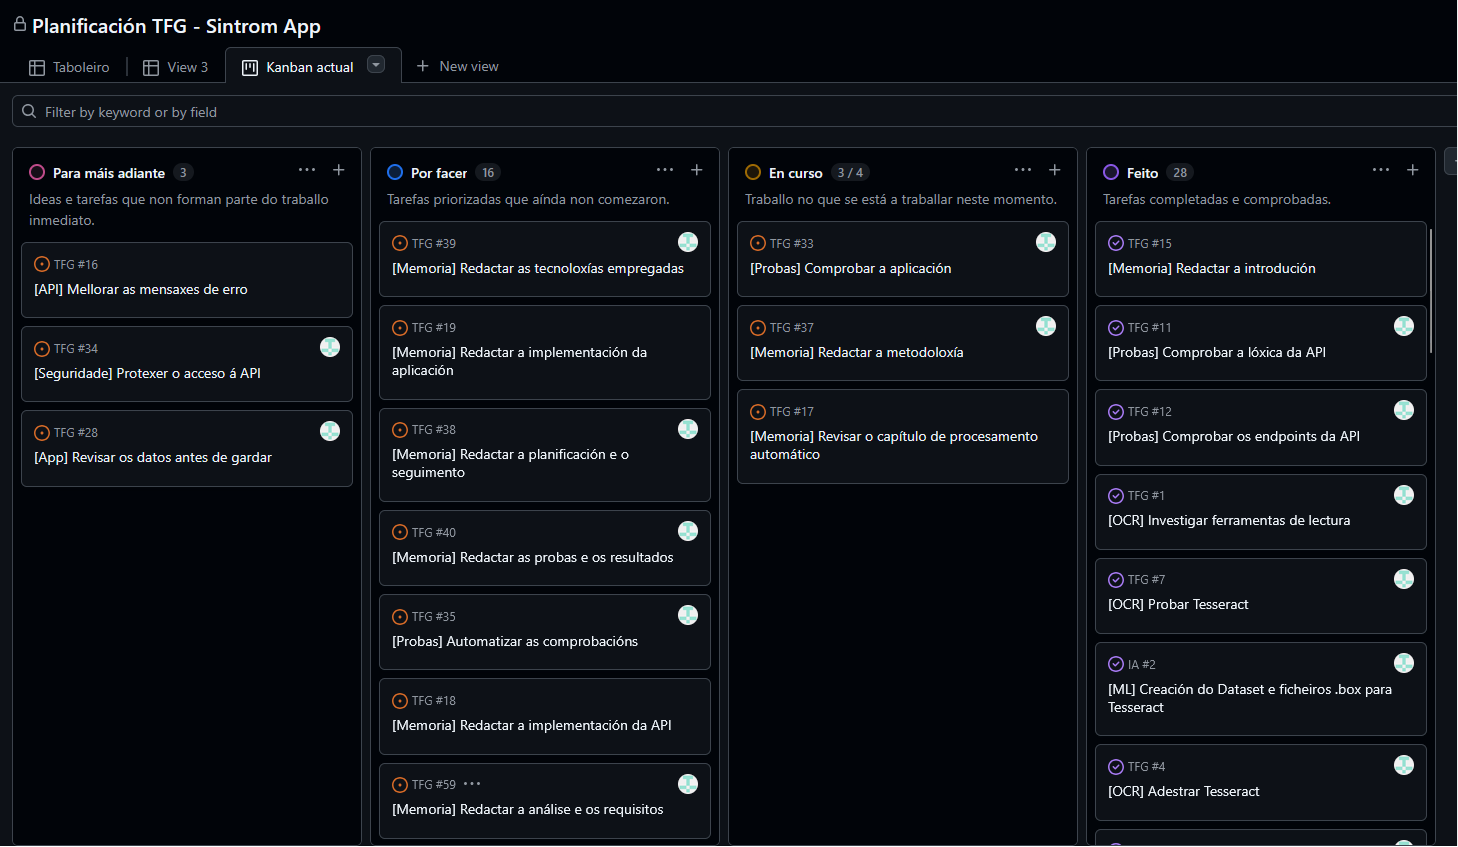
\includegraphics[width=1\linewidth]{imaxes/02-Metodoloxía/taboleiro-kanban.png}
     \caption{Estado do taboleiro Kanban o 20 de Xullo de 2026.}
     \label{fig:taboleiro-kanban}
 \end{figure}
 
\begin{figure}[h!]
    \centering
    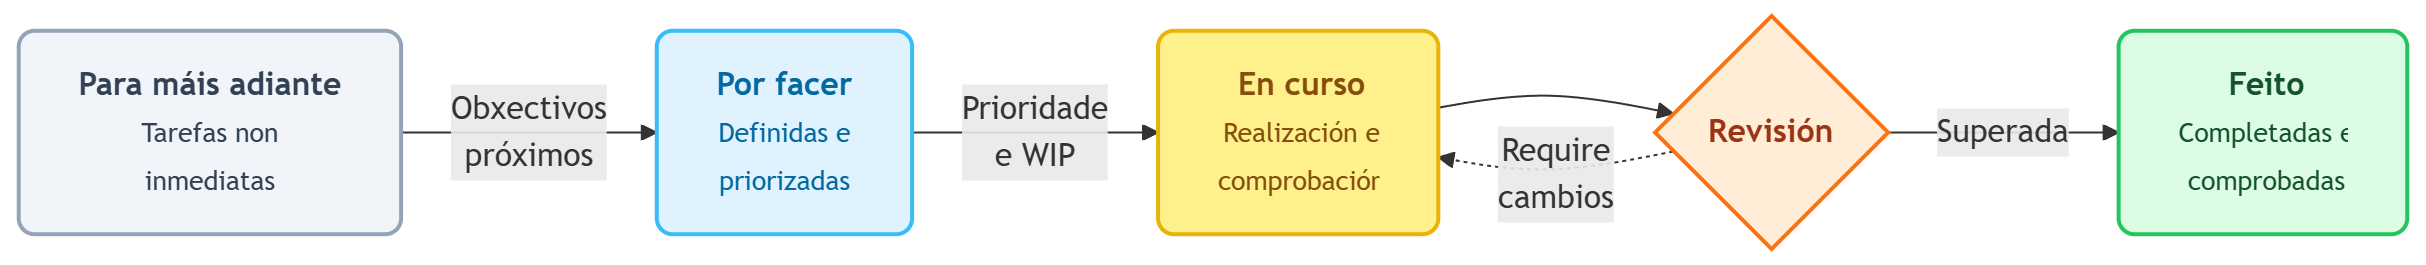
\includegraphics[width=1\linewidth]{imaxes/02-Metodoloxía/diagrama-kanban.png}
    \caption{Diagrama do fluxo de tarefas no taboleiro Kanban.}
    \label{fig:diagrama-kanban}
\end{figure}

\subsection{Límite de traballo en curso}

Estableceuse un límite de traballo en curso, ou límite WIP (\textit{Work In Progress}), de \textbf{catro tarefas}. O seu obxectivo foi favorecer a finalización das tarefas iniciadas antes de comezar outras novas.

Escolleuse este valor porque permitía manter activas tarefas de distintas áreas do proxecto sen acumular un número excesivo de actividades abertas. No cómputo do límite incluíanse tamén as tarefas pendentes de revisión, validación ou
desbloqueo, polo que non implicaba que se desenvolvesen catro tarefas simultaneamente.

Cando se alcanzaba o límite, priorizábase a finalización, integración ou desbloqueo das tarefas existentes antes de iniciar outras novas.


\subsection{Organización e priorización das tarefas}

Cada tarefa do taboleiro representouse mediante unha \textit{issue} de GitHub. Nela recollíanse a descrición do traballo, os criterios de aceptación, a prioridade, as etiquetas e, cando correspondía, as relacións con outras tarefas ou \textit{pull requests}.

Na Figura~\ref{fig:exemplo-tarefa} preséntase unha das tarefas do proxecto, na que se poden observar algúns destes elementos.

\begin{figure}[h!]
    \centering
    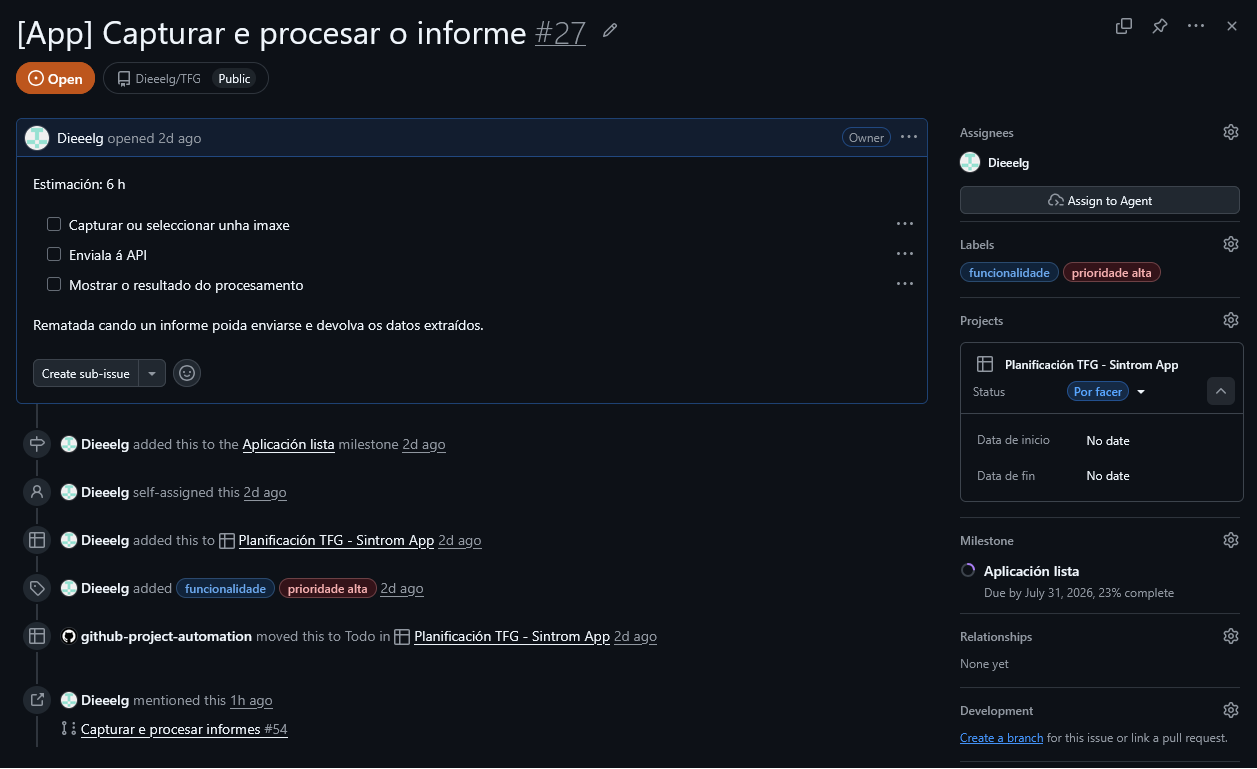
\includegraphics[width=1\linewidth]{imaxes/02-Metodoloxía/exemploTarefa.png}
    \caption{Exemplo dunha tarefa do proxecto.}
    \label{fig:exemplo-tarefa}
\end{figure}
\FloatBarrier

Para representar a prioridade das tarefas empregáronse tres etiquetas:

\begin{itemize}
    \item \textbf{Prioridade alta}: tarefas que debían realizarse canto antes, especialmente cando bloqueaban o fluxo principal ou outras actividades.
    \item \textbf{Prioridade media}: tarefas importantes, pero que non impedían continuar co desenvolvemento.
    \item \textbf{Prioridade baixa}: tarefas que podían pospoñerse ata completar as funcionalidades principais.
\end{itemize}

As tarefas priorizáronse atendendo principalmente á súa importancia para completar o fluxo principal, ás dependencias con outras tarefas, á dificultade e á incerteza técnica, á proximidade do fito ao que pertencían e á existencia de bloqueos que impedisen avanzar noutras funcionalidades.

Deste xeito, as funcionalidades necesarias para procesar unha folla de tratamento, gardar os datos, consultar a pauta e confirmar unha toma recibiron unha prioridade superior ás melloras visuais. Do mesmo xeito, unha corrección que bloqueaba varias tarefas tiña prioridade sobre unha funcionalidade independente que podía incorporarse máis adiante.

O taboleiro revisouse periodicamente e ao finalizar cada incremento. Durante estas revisións actualizáronse os estados e as prioridades das tarefas, e identificáronse posibles bloqueos ou actividades que permanecían demasiado tempo en curso.

Cando unha tarefa resultaba demasiado extensa ou combinaba cambios non relacionados, dividíase en tarefas máis pequenas para facilitar a súa estimación, desenvolvemento e comprobación.

\section{Aplicación de GitFlow ao control de versións}
\label{sec:gitflow}

Para xestionar as distintas versións do código empregáronse Git e GitHub xunto cunha adaptación simplificada de GitFlow. Este modelo permite separar o código estable do código en desenvolvemento e realizar cada cambio nunha rama independente antes de integralo~\cite{DriessenGitFlow}.

No proxecto utilizáronse os seguintes tipos de ramas:
\begin{itemize}
    \item \textit{master}: mantívose como referencia estable do proxecto.
    \item \textit{develop}: empregouse como rama de integración das funcionalidades xa comprobadas.
    \item \textit{feature/nome-da-tarefa}: utilizouse para desenvolver novas funcionalidades. Algúns exemplos son \textit{feature/calendario},  \textit{feature/confirmar-tomas} ou \textit{feature/vincular-coidador}
    \item \textit{fix/nome-do-problema}: empregouse para correccións concretas, como \textit{fix/configuracion-local} e \textit{fix/datos-centros}.
\end{itemize}

\begin{figure}[h!]
    \centering
    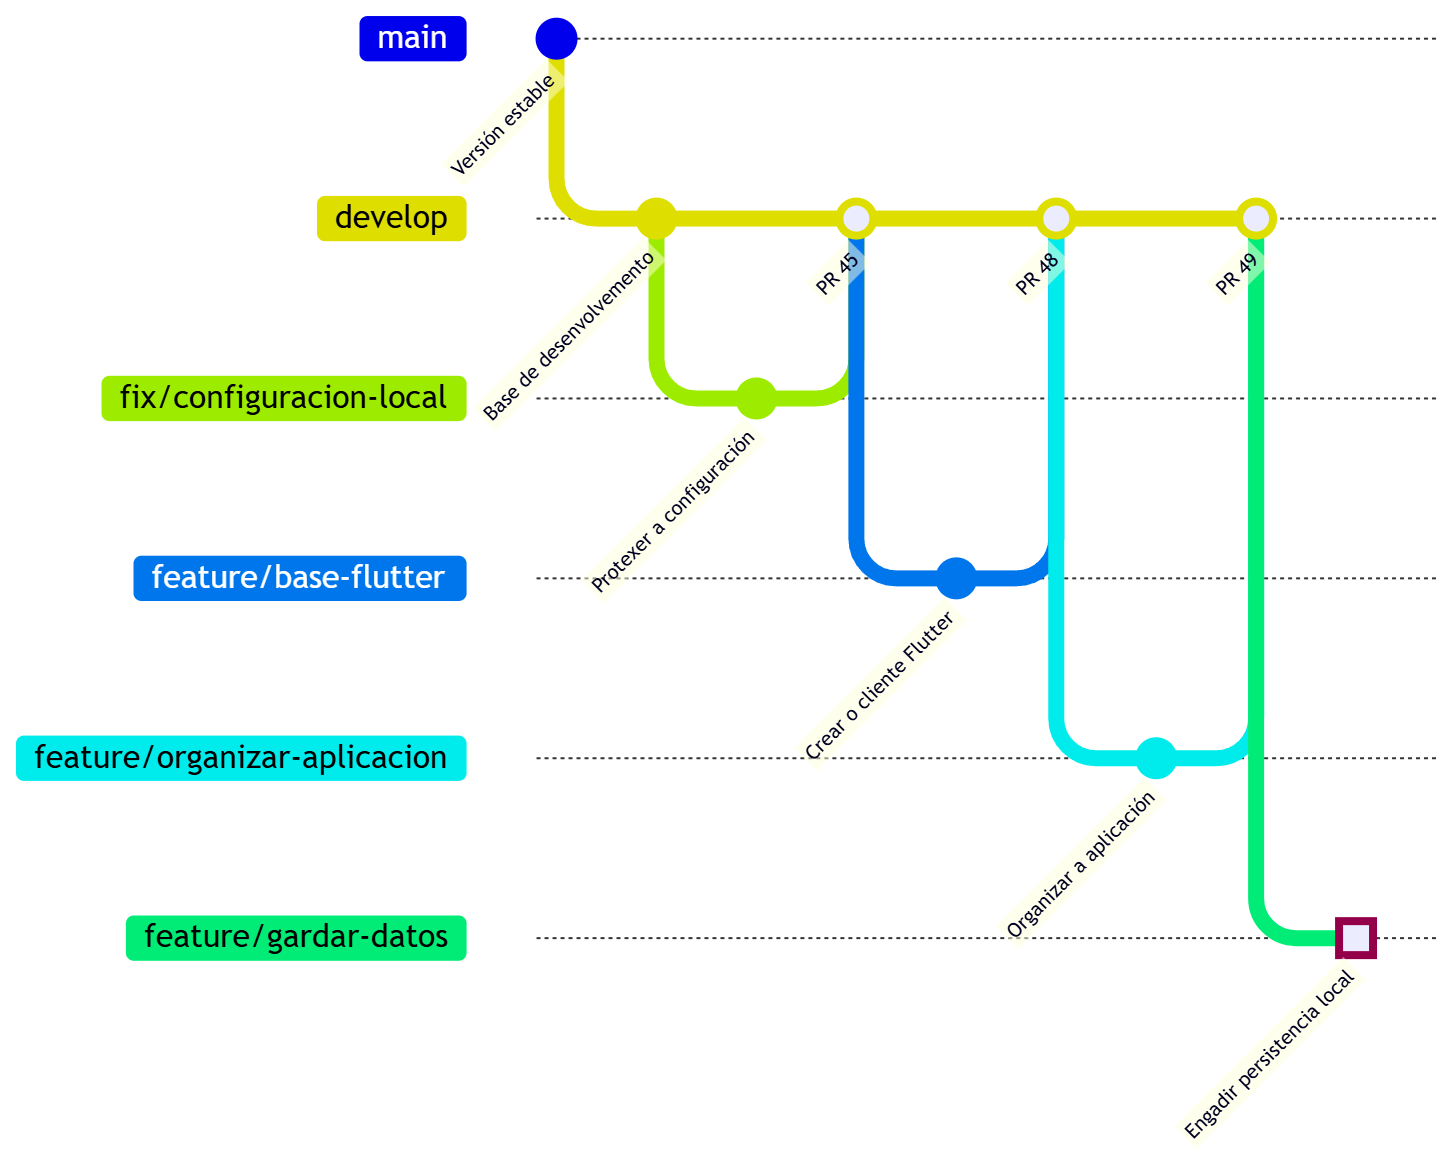
\includegraphics[width=0.7\linewidth]{imaxes/02-Metodoloxía/diagrama-gitflow.png}
    \caption{Adaptación de GitFlow empregada no proxecto.}
    \label{fig:diagrama-gitflow}
\end{figure}

Para ilustrar este fluxo de traballo, a Figura~\ref{fig:diagrama-gitflow} mostra unha representación visual dalgunhas das ramas empregadas no proxecto. No grafo pódese observar a rama principal (\textit{main}) e a base de desenvolvemento (\textit{develop}), así como exemplos reais do historial. As ramas resoltas, como \textit{fix/configuracion-local} ou \textit{feature/base-flutter}, parten de \textit{develop} e intégranse de novo a través das súas respectivas \textit{pull requests} (como as PR 45, PR 48 e PR 49). Pola contra, o traballo en curso, como a rama \textit{feature/gardar-datos}, mantense illado ata a súa finalización.


As ramas de funcionalidades e correccións creábanse a partir de \textit{develop}.  O código nunca se modificou directamente sobre as ramas principais, garantindo así o illamento de cada tarefa. Durante o desenvolvemento, os cambios rexistráronse aplicando a convención de \textit{commits} semánticos (empregando prefixos como \textit{feat:}, \textit{fix:}, \textit{refactor:} ou \textit{chore:}). Isto permitiu manter un historial lexible e descritivo que indica claramente o propósito de cada modificación.

Unha vez rematada unha tarefa, a rama correspondente publicábase no repositorio remoto e abríase unha \textit{pull request} cara a rama \textit{develop}. Este mecanismo empregouse aínda que o proxecto fose desenvolvido por unha única persoa. Neste contexto non proporcionaban unha revisión independente, pero si ofrecían un punto de control antes de modificar \textit{develop}. Ademais, permitían consultar a descrición do cambio, os commits incluídos, os ficheiros modificados e a relación coa tarefa correspondente.

Na Figura~\ref{fig:exemplo-pull-request} móstrase un exemplo deste proceso, correspondente á integración mediante \textit{pull request} dunha das tarefas de desenvolvemento.

\begin{figure}[h!]
    \centering
    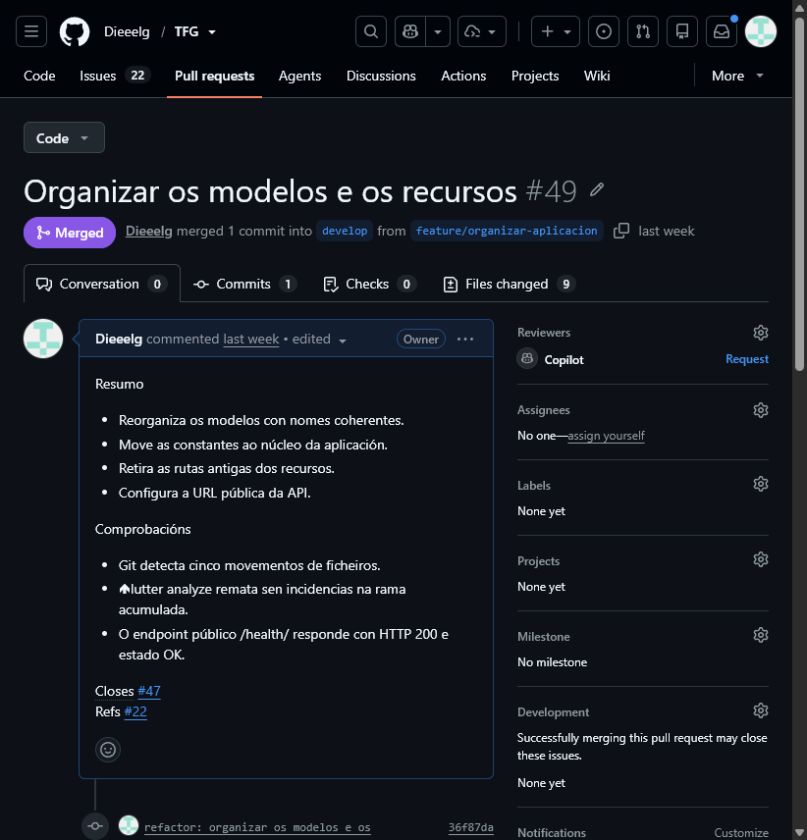
\includegraphics[width=0.7\linewidth]{imaxes/02-Metodoloxía/exemplo-pull-request.png}
    \caption{Integración dunha rama de funcionalidade en \textit{develop} mediante unha \textit{pull request}.}
    \label{fig:exemplo-pull-request}
\end{figure}



A principal diferenza desta adaptación con respecto ao modelo orixinal foi a omisión das ramas de \textit{release} e \textit{hotfix}. Dado que o proxecto non requiría manter simultaneamente varias versións publicadas en produción, esta simplificación permitiu conservar as vantaxes principais do illamento de código sen introducir unha complexidade innecesaria no fluxo de traballo.

\section{Xustificación da metodoloxía}

A combinación dun desenvolvemento incremental e iterativo cun taboleiro Kanban resultou axeitada para as características e necesidades do proxecto. Durante as primeiras etapas existía unha elevada incerteza sobre a viabilidade da extracción automática dos datos e sobre a tecnoloxía máis axeitada para realizala. Por este motivo, resultaba difícil establecer desde o inicio unha planificación pechada ou estimar con precisión a duración das tarefas de investigación e experimentación.

O enfoque incremental permitiu avanzar por etapas e reducir progresivamente esta incerteza. Primeiro estudouse a viabilidade da extracción automática, despois seleccionouse unha tecnoloxía e desenvolveuse unha primeira versión funcional da API e, finalmente, construíuse a aplicación móbil. Cada incremento proporcionou un resultado comprobable que serviu como base para continuar co desenvolvemento.

O carácter iterativo permitiu revisar solucións xa desenvolvidas cando se obtiveron novos resultados. As decisións relacionadas coa extracción dos datos, a organización da API e o funcionamento da aplicación fóronse modificando e refinando a medida que se coñecían mellor a estrutura das follas de tratamento e as necesidades do sistema.

Non se aplicou Scrum de maneira estrita porque a organización do traballo en sprints de duración fixa non se considerou a opción máis axeitada para unhas tarefas cunha duración e uns resultados difíciles de prever. En cambio, Kanban permitiu manter un fluxo continuo, modificar as prioridades segundo os avances realizados e incorporar novas tarefas cando se detectaban necesidades ou problemas.

O taboleiro proporcionou unha representación visual do estado do proxecto, diferenciando as tarefas pendentes, as que se atopaban en desenvolvemento e as que xa foran comprobadas. O límite de traballo en curso favoreceu a finalización das tarefas iniciadas antes de abrir novas liñas de traballo e permitiu identificar aquelas que permanecían pendentes de revisión ou validación.

No relativo á xestión do código, o uso de GitFlow axudou a manter o traballo moito máis organizado. O feito de programar cada tarefa nunha rama separada e usar \textit{pull requests} obrigou a facer unha revisión persoal de cada cambio antes de integralos no código principal. Ademais, o emprego de \textit{commits} semánticos permitiu crear un historial moito máis claro, onde é moi doado entender os pasos que se foron dando.

Como principal limitación, ao tratarse dun proxecto individual non se contou cunha revisión independente continua do traballo realizado. Para reducir este risco combinouse a auto-revisión nas \textit{pull requests} co uso de criterios de aceptación, listas de comprobación e comprobacións técnicas e funcionais antes de integrar os cambios e considerar completadas as tarefas.